\documentclass[aspectratio=169]{beamer}
\usetheme[numbering=fraction]{metropolis}           % Use metropolis theme;
%\usepackage{FiraSans}

\usepackage[absolute,overlay]{textpos}
\usepackage[T1]{fontenc}
\usepackage{setspace}
\usepackage{xcolor}
\usepackage{caption}

%%%%%%%%%%%%%%%%%%%%%%%
% Background setup
\pgfdeclareimage[width=\paperwidth,height=\paperheight]{bg2}{figs/bg2} % Declare background image

\defbeamertemplate*{background canvas}{mydefault}
  {%
    \ifbeamercolorempty[bg]{background canvas}{}{\color{bg}\vrule width\paperwidth height\paperheight}% copied beamer default here
  }
  \defbeamertemplate*{background canvas}{bg}
 {%
   \color{mDarkTeal}\vrule width\paperwidth height\paperheight% added bg color
 }

 \defbeamertemplate*{background canvas}{image}
{%
    \begin{tikzpicture}
        \useasboundingbox (0,0) rectangle (\the\paperwidth, \the\paperheight);
        \pgftext[at=\pgfpoint{0cm}{0cm}, left, base]{\pgfuseimage{bg2}};
    \end{tikzpicture}
}

 \BeforeBeginEnvironment{frame}{%
   \setbeamertemplate{background canvas}[mydefault]%
 }

 \makeatletter
 \define@key{beamerframe}{bg}[true]{%
   \setbeamertemplate{background canvas}[bg]%
 }

 \makeatletter
\define@key{beamerframe}{image}[true]{%
  \setbeamercovered{invisible}%
  \setbeamertemplate{background canvas}[image]%
}

%%%%%%%%%%%%%%%%%%%%%%
%% General setup
%% Fonts and typography
\setbeamerfont{title}{size=\huge,%
                      series=\bfseries}
\setbeamerfont*{subtitle}{size=\Large,%
                          series=\bfseries}
\setbeamerfont{author}{size=\large}
\setbeamerfont{date}{size=\large}
\setbeamerfont{frametitle}{size=\Large,%
                           series=\bfseries}

% color
\setbeamercolor{titlelike}{use=palette primary, parent=palette primary}
\setbeamercolor{author}{use=palette primary, parent=palette primary}
\setbeamercolor{date}{use=palette primary, parent=palette primary}
\setbeamercolor{institute}{use=palette primary, parent=palette primary}
\setbeamercolor{structure}{use=palette primary, parent=palette primary}

\setbeamertemplate{title}{
  \flushleft%
  \setstretch{.85}%
  \inserttitle%
  \par%
  \vspace*{0.1em}
 }
 \setbeamertemplate{subtitle}{
  \raggedright%
  \setstretch{.85}%
  \insertsubtitle%
  \par%
  \vspace*{0.5em}
}

% Title page frame
\setbeamertemplate{title page}{
%\pgfdeclareimage[height=0.6cm]{logo}{UdeS_blanc} % Declare first Logo
%\pgfdeclareimage[height=0.45cm]{logo2}{IELab} % Declare second Logo
  \begin{minipage}[b][\paperheight]{10cm}
    \ifx\inserttitlegraphic\@empty\else\usebeamertemplate*{title graphic}\fi
    \vfill%
    \ifx\inserttitle\@empty\else\usebeamertemplate*{title}\fi
    \ifx\insertsubtitle\@empty\else\usebeamertemplate*{subtitle}\fi
    %\usebeamertemplate*{title separator} % puts a line under the title
    \ifx\beamer@shortauthor\@empty\else\usebeamertemplate*{author}\fi
    \ifx\insertdate\@empty\else\usebeamertemplate*{date}\fi
    \ifx\insertinstitute\@empty\else\usebeamertemplate*{institute}\fi
    %\vfill%
    \vspace*{8mm}
    %\pgfuseimage{logo} % Use logo
    %\newcommand\mybar{\kern1pt\rule[-\dp\strutbox]{.8pt}{.7cm}{\hspace{2mm}}\kern1pt} % White bar
    %\textcolor{white}{\mybar{\pgfuseimage{logo2}}} % Second logo
    %\vfill
    \vspace*{15mm}
  \end{minipage}
}

%%%%%%%%%%%%%%%%%%%%%%%%%%%
% Examples

%% Makes title slide with only background defined color
  %\begin{frame}[bg]
    %\titlepage
  %\end{frame}
%% Makes a title slide with background + image
  %\begin{frame}[image]
    %\titlepage
  %\end{frame}
%% Makes also a title slide with background + image
  %\maketitle

%%%%%%%%%%%%%%%%%%%%%%%%%%%

\title{Aire de distribution et changements climatiques:}
\subtitle{Comment les interactions biotiques moduleront-elles la réponse?}
%\date{\today}
\author{Victor Cameron}




\begin{document}

%% Effect of climate change on the co-distribution of forest trees and passerine birds
\maketitle % make title produces formated title slide

%%% keys
%1. Le titre
%2. Structure spéciale: Étude théorique = exploration
%3. Pas d'hypothèse
%4. Cette présentation a pour but de présenter mon projet

%%%%%%%%%%%%%%%%%%%%%%%%%%%%%%%%%%%%%%%%%%%%%%%%%%%%%%%%%%%%%%%%%%%%%%%%%%%%%%%%%
%%% Contexte

{%
\setbeamertemplate{frame footer}{Ferrarini \textit{et al}. 2017}
\begin{frame}{Contexte\hskip 1em \mdseries{\textcolor{lightgray}{Les limites de distribution}}}

  Un \textbf{déplacement des aires de distribution} est attendu dans les 100 prochaines années

  \begin{figure}
  	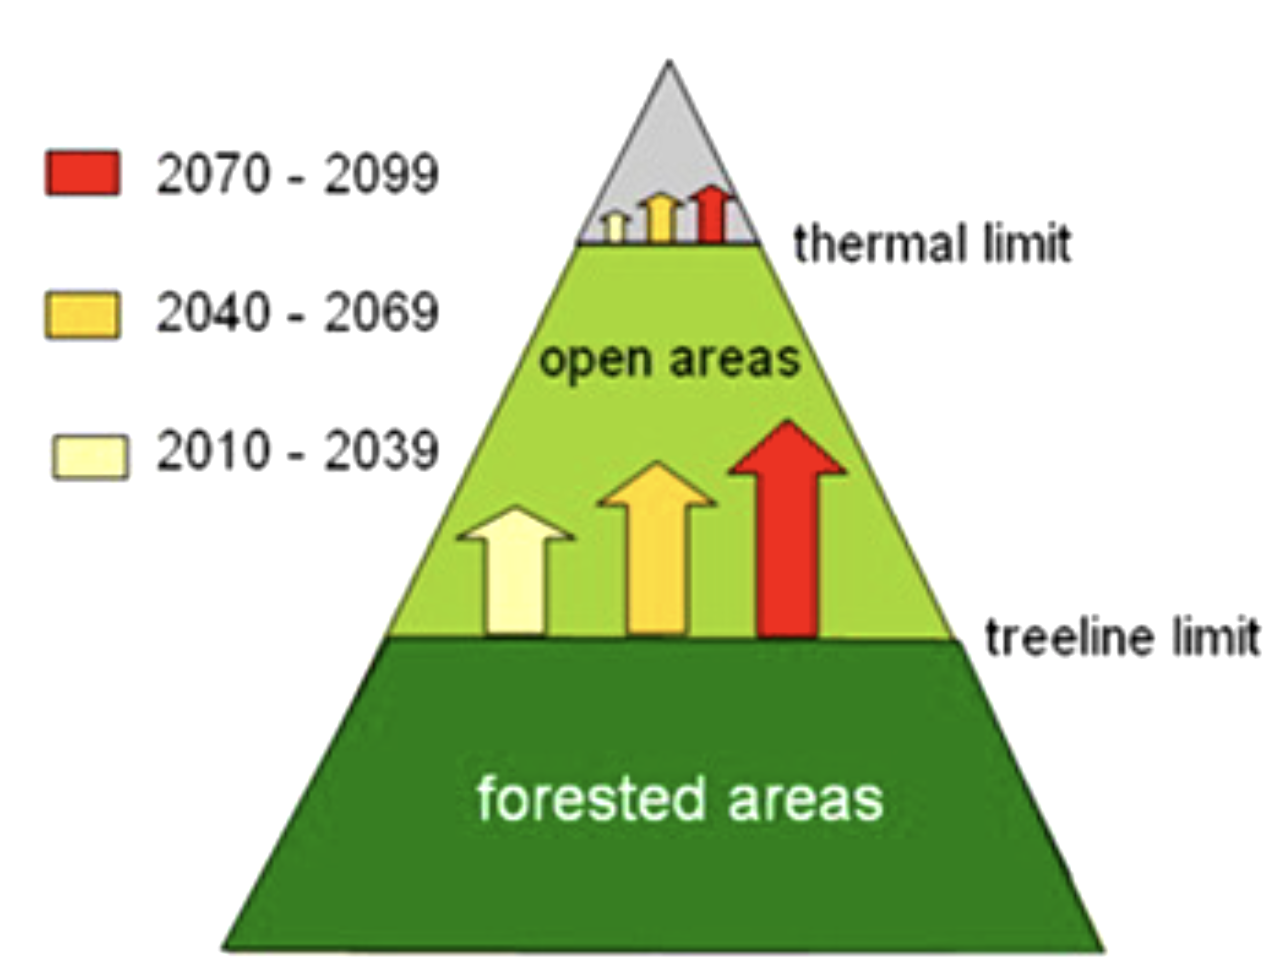
\includegraphics[height=.60\paperheight]{figs/Ferrarini.png}
    %\caption*{ \textbf{Eveloppe climatique de l'érable à sucre présente et projetée (2071-2100)}}
  \end{figure}

\end{frame}
}

%%% L'aire de distribution d'une espèce est limitée
%%% Une connaissance des processus limitant l'aire de distribution est fondamentale pour prévoir les distributions dans le futur

%%%%%%%%%%%%%%%%%%%%%%%%%%%%%%%%%%%%%%%%%%%%%%%%%%%%%%%%%%%%%%%%%%%%%%%%%%%%%%%%%
%%% Contexte

{%
\setbeamertemplate{frame footer}{}
\begin{frame}{Contexte\hskip 1em \mdseries{\textcolor{lightgray}{Les limites de distribution}}}

  1. L'emplacement des limites de distribution est \textbf{sensible au climat}

  \begin{figure}
  	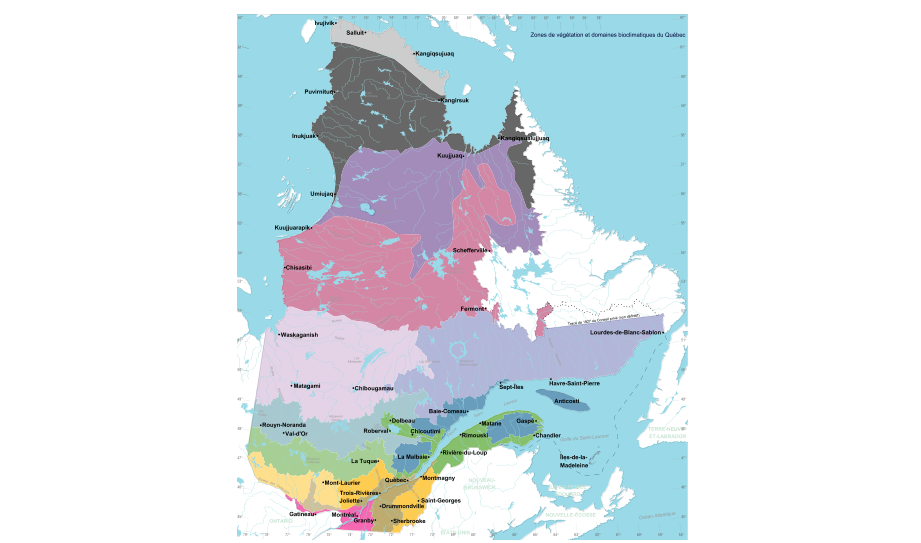
\includegraphics[height=.65\paperheight]{figs/bioclim.png}
    %\caption*{ \textbf{Distribution présente et projetée}}
  \end{figure}

\end{frame}
}

%%% On s'attend à trouver les espèces là où le climat est favorable et absentes là où le climat est défavorable
%%%

%%%%%%%%%%%%%%%%%%%%%%%%%%%%%%%%%%%%%%%%%%%%%%%%%%%%%%%%%%%%%%%%%%%%%%%%%%%%%%%%%
%%% Contexte

{%
\setbeamertemplate{frame footer}{}
\begin{frame}{Contexte\hskip 1em \mdseries{\textcolor{lightgray}{Projection des futures distributions}}}

  2. On s'attend à ce que les enveloppes climatiques se \textbf{déplacent vers le nord ou vers des altitudes plus élevées} en réponse aux changements climatiques

  \begin{figure} % Photos de passeraux associés à divers types de forêts
    % Paruline azurée (ou couronnée?) est associée aux érablières

  \end{figure}

\end{frame}
}

%%% Les espèces réactives pourront suivre le déplacement de leur enveloppe climatique
%%% Les espèces moins réactives accuseront un retard
%%% Il a été observé que la végétation accuse un retard sur le déplacement son enveloppe climatique
%%% Différents temps de réactions peuvent faire que des espèces qui co-occurent présentement ne co-occurent plus dans le futur

%%%%%%%%%%%%%%%%%%%%%%%%%%%%%%%%%%%%%%%%%%%%%%%%%%%%%%%%%%%%%%%%%%%%%%%%%%%%%%%%%
%%% Contexte

{%
\setbeamertemplate{frame footer}{McKenney \textit{et al}. 2007, Talluto \textit{et al}. 2017}
\begin{frame}[t]{Contexte\hskip 1em \mdseries{\textcolor{lightgray}{Difficultés reliées au contexte}}}

  Les \textbf{modèles de distribution d'espèces} (SDMs) sont des modèles mathématiques qui corrèlent la \emph{distribution} d'une espèce avec des \emph{données climatiques}

  \begin{columns}[]
    \begin{column}{0.5\textwidth}
      \begin{figure}
        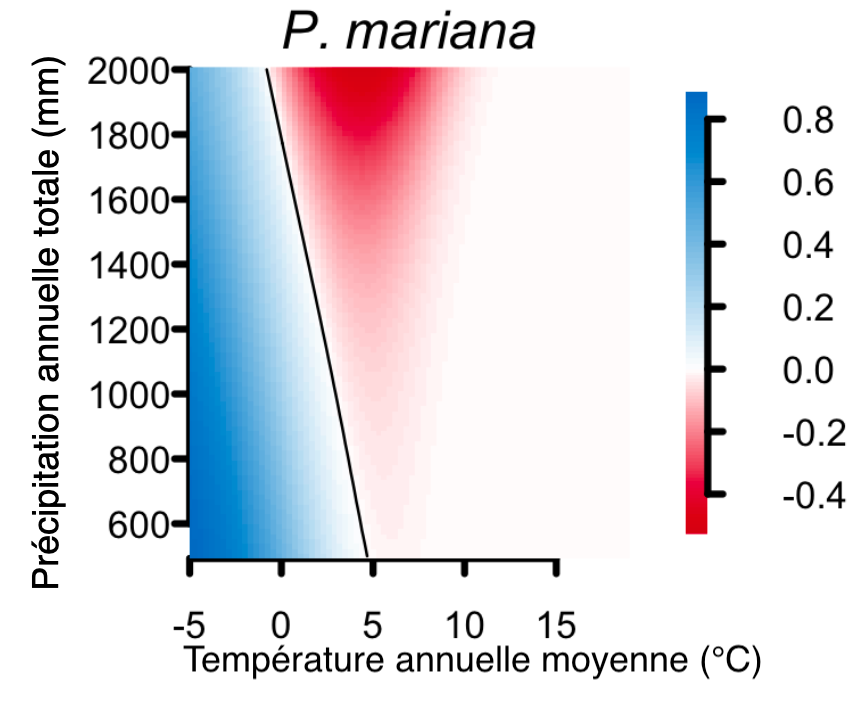
\includegraphics[height=.65\textwidth]{figs/Talluto2.png}
      \end{figure}
    \end{column}

    \begin{column}{0.5\textwidth}
      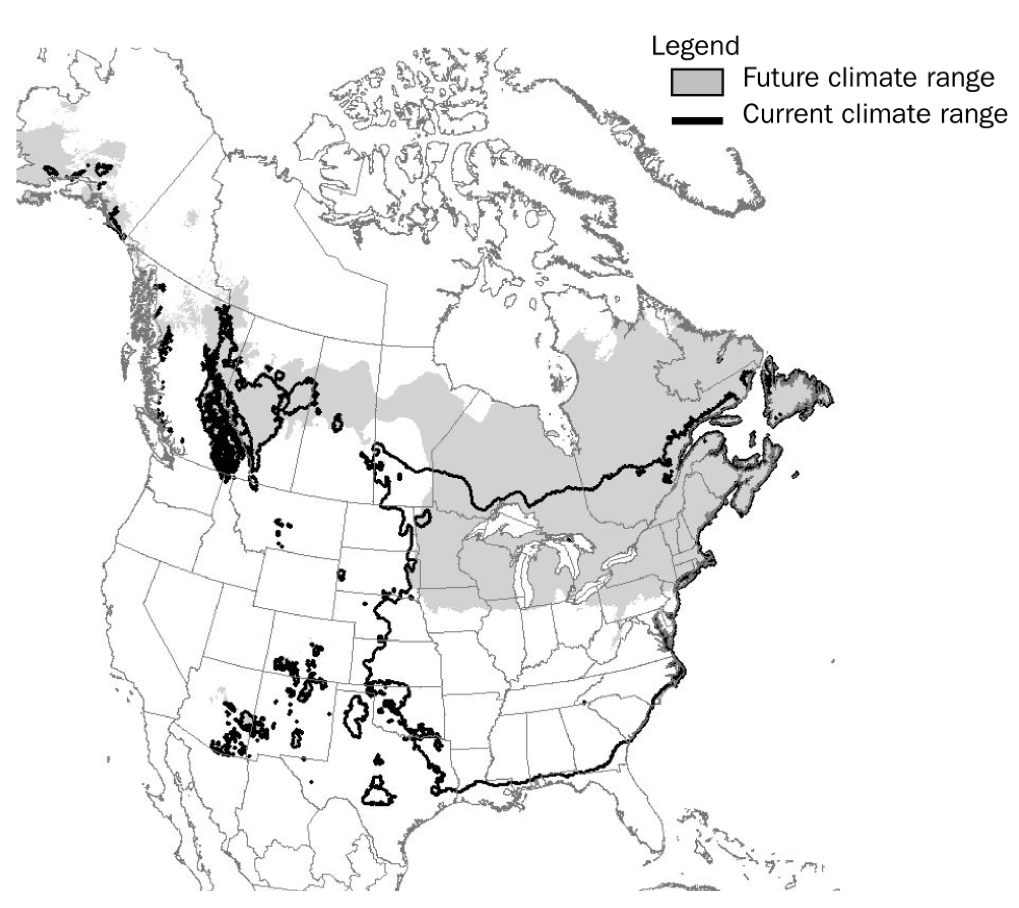
\includegraphics[height=.65\textwidth]{figs/mckenney.png}
    \end{column}
  \end{columns}

\end{frame}
}

%% Les SDMs sontdes modèles mathématiques

%%%%%%%%%%%%%%%%%%%%%%%%%%%%%%%%%%%%%%%%%%%%%%%%%%%%%%%%%%%%%%%%%%%%%%%%%%%%%%%%%
%%% Contexte

\begin{frame}{Contexte\hskip 1em \mdseries{\textcolor{lightgray}{Difficultés reliées au contexte}}}

  Les \textbf{modèles de distribution d'espèces} (SDMs) font de nombreuses suppositions:
    \begin{itemize}
      \item Distribution à l'équilibre avec l'enveloppe climatique;
      \item Absence de démographie;
      \item Absence de limite de dispersion;
      \item Absence d'interaction biotique;
      \item Réponse linéaire et instantannée au changement climatique.
    \end{itemize}

\end{frame}

%% Les outils actuels pour prédire l'impact des changements climatiques sur la distribution des espèces sont limités par l'absence de processus écologiques fondamentaux.
%% Def interaction: l'effet qu'une espèce  a sur le fitness d'une autre espèce (taux de croissance de population): pred-proie, habitat-utilisateur

%%%%%%%%%%%%%%%%%%%%%%%%%%%%%%%%%%%%%%%%%%%%%%%%%%%%%%%%%%%%%%%%%%%%%%%%%%%%%%%%%
% % % Contexte

\begin{frame}{Contexte\hskip 1em \mdseries{\textcolor{lightgray}{Difficultés reliées au contexte}}}

  %% Quand on s'intéresse au changements d'aire de répartition d'une communauté, certains processus sont à prendre en considérations:
  Les espèces qui \textbf{co-occurent}:
  \begin{itemize}
    \item Ont différents temps de réponse au changement climatique;
    \item Ne se reproduisent pas au même rythme;
    \item N'ont pas toutes la même capacité de dispersion;
    \item Interagissent.
  \end{itemize}

  \alert{Ces processus peuvent modifier la relation entre le climat et la distribution des espèces}

\end{frame}

%% Les processus peuvent avoir des conséquences inatendues sur les futures distributions

%%%%%%%%%%%%%%%%%%%%%%%%%%%%%%%%%%%%%%%%%%%%%%%%%%%%%%%%%%%%%%%%%%%%%%%%%%%%%%%%%
% % %

\begin{frame}{Objectifs\hskip 1em \mdseries{\textcolor{lightgray}{Subtitle}}}

  \textbf{Objectif général:} Évaluer les impacts d'un changement climatique sur la distribution régionale et la persistance d'une espèce en intéraction avec son habitat.

  \textbf{\\Pourquoi?}
  \begin{enumerate}
    \item Développer un nouvel outil théorique pour améliorer la prédiction des impacts du changement climatique sur la distribution des espèces;
    \item Évaluer l'impact des interactions biotiques sur la réaction des aires de distribution au changement climatique.
  \end{enumerate}

\end{frame}

%%%%%%%%%%%%%%%%%%%%%%%%%%%%%%%%%%%%%%%%%%%%%%%%%%%%%%%%%%%%%%%%%%%%%%%%%%%%%%%%%
% % %

{%
\setbeamertemplate{frame footer}{Pulliam 2000, Sandoro 2008}
\begin{frame}{Théorie \hskip 1em \mdseries{\textcolor{lightgray}{Interactions biotiques}}}

Les \textbf{interactions biotiques} sont d'importantes forces modulaires des limites de distribution à \emph{petites et à grandes échelles spatiales}

\begin{figure}
  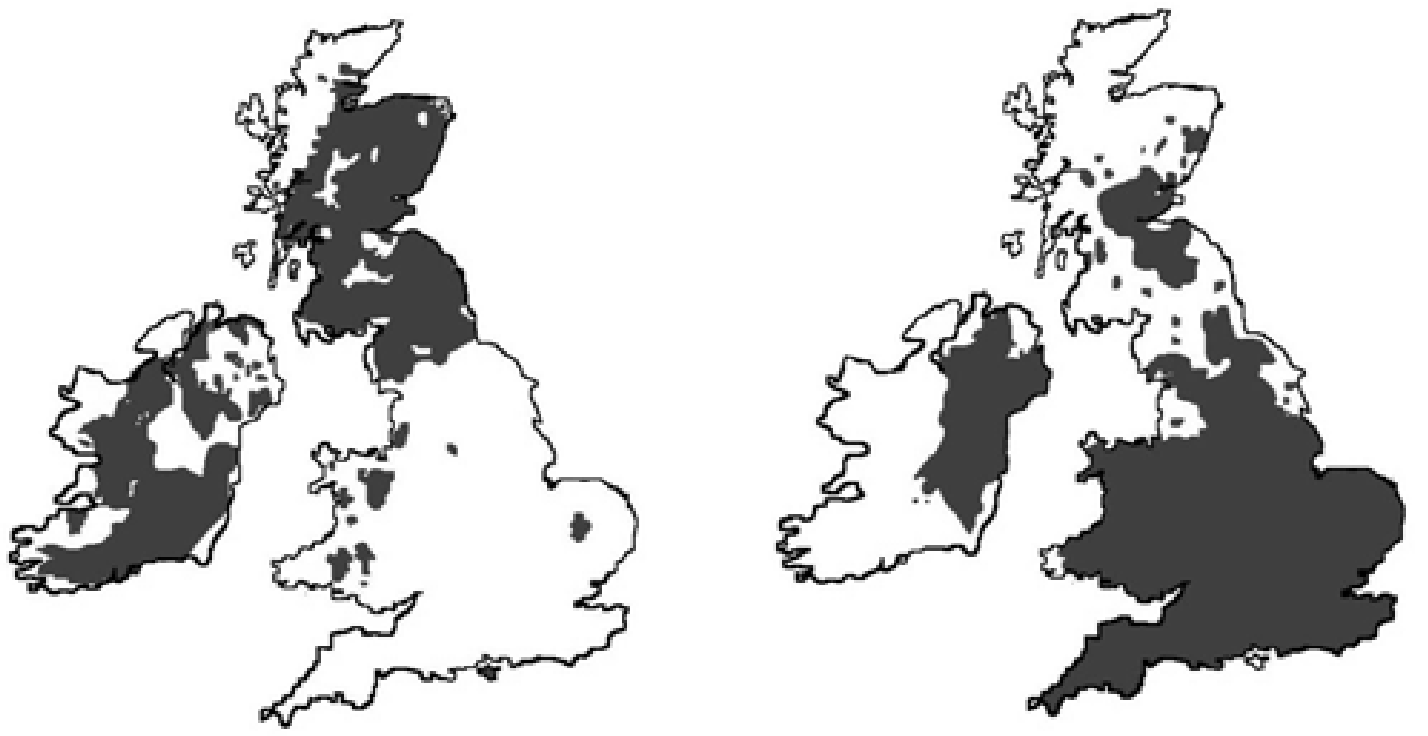
\includegraphics[height=.60\paperheight]{figs/Sandoro.png}
  %\caption*{ \textbf{}}
\end{figure}

\end{frame}
}

%% Interaction biotiques: effet d'une espèce sur le fitness (taux de croissance) d'une autre espèce
%% Historiquement: Conditions climatiques importantes à large échelle, et les interactions à l'échelle locale
%% Little interest in the study of biotic interactions at large geographical scales: important need for methods to account for interactions in future predictions

%%%%%%%%%%%%%%%%%%%%%%%%%%%%%%%%%%%%%%%%%%%%%%%%%%%%%%%%%%%%%%%%%%%%%%%%%%%%%%%%%
% % %

{%
\setbeamertemplate{frame footer}{Pulliam 2000, Godsoe \textit{et al}. 2017}
\begin{frame}{Théorie\hskip 1em \mdseries{\textcolor{lightgray}{Niche}}}

  %b,d --> c,e,h  (disponibilité d'habitat: montrer schéma que j'ai fait)
  $$r(E,R) > b(E,R) - d(E,R)$$ $$\lambda (E,H) > c(E,H) - e(E,H)$$

  \begin{figure}
  	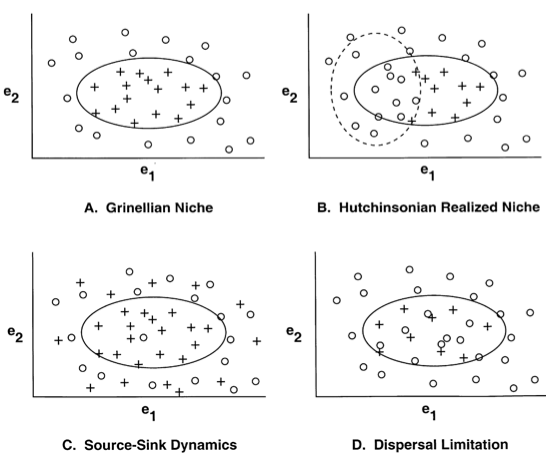
\includegraphics[height=.65\paperheight]{figs/pulliam.png}
    %\caption*{ \textbf{}}
  \end{figure}

  \begin{figure}
  	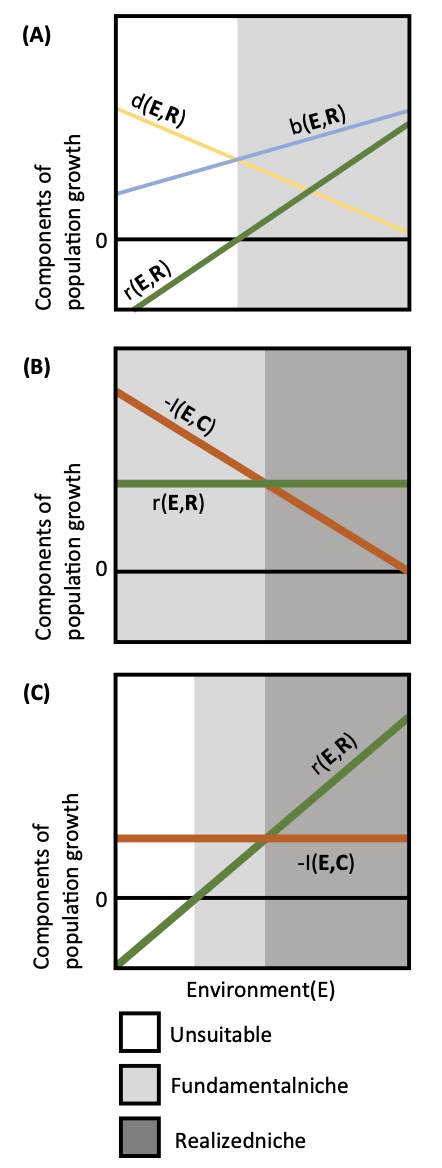
\includegraphics[height=.65\paperheight]{figs/godsoe.png}
    %\caption*{ \textbf{}}
  \end{figure}

\end{frame}
}

%% Godsoe: approche les limites de distribution avec la théorie de la niche (r>b-d)
%% Besoin d'une perspective régionale (\lambda>c-e --> suget de ma maitrise (montrer les schémas que j'ai fait)
%% disponibilité d'habitat

%%%%%%%%%%%%%%%%%%%%%%%%%%%%%%%%%%%%%%%%%%%%%%%%%%%%%%%%%%%%%%%%%%%%%%%%%%%%%%%%%
% % %

\begin{frame}{Théorie\hskip 1em \mdseries{\textcolor{lightgray}{Métapopulations}}}



\end{frame}

%%%%%%%%%%%%%%%%%%%%%%%%%%%%%%%%%%%%%%%%%%%%%%%%%%%%%%%%%%%%%%%%%%%%%%%%%%%%%%%%%
% % %

{%
\setbeamertemplate{frame footer}{Svenning \textit{et al}. 2014}
\begin{frame}{Théorie\hskip 1em \mdseries{\textcolor{lightgray}{Range shifts}}}

  \begin{figure}
  	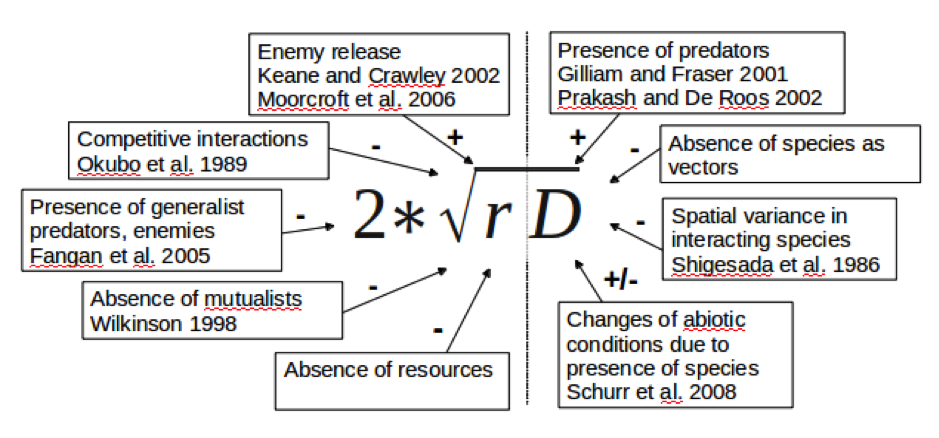
\includegraphics[height=.65\paperheight]{figs/svenning.png}
    %\caption*{ \textbf{}}
  \end{figure}

\end{frame}
}

%%%%%%%%%%%%%%%%%%%%%%%%%%%%%%%%%%%%%%%%%%%%%%%%%%%%%%%%%%%%%%%%%%%%%%%%%%%%%%%%%
% % %

\begin{frame}{Étude de cas\hskip 1em \mdseries{\textcolor{lightgray}{Subtitle}}}

  Pour aider à relier les concepts que j'ai presenté et les objectifs que je me posés

\end{frame}

%%%%%%%%%%%%%%%%%%%%%%%%%%%%%%%%%%%%%%%%%%%%%%%%%%%%%%%%%%%%%%%%%%%%%%%%%%%%%%%%%
% % %

\begin{frame}{Objectifs\hskip 1em \mdseries{\textcolor{lightgray}{Subtitle}}}

  \textbf{Objectif général:} Évaluer les impacts d'un changement climatique sur la distribution régionale de la give de Bicknell et sa persistance.

  \textbf{\\Objectifs secondaires:}
    \begin{enumerate}
      \item Un premier objectif faisant référence à la capacité de support de la métapopulation (effet à grande échelle)
      \item Un deuxième pbjectif faisant référence à la dynamique de la métapop (vitesse de réaction; phase transiante)
    \end{enumerate}

\end{frame}

%%%%%%%%%%%%%%%%%%%%%%%%%%%%%%%%%%%%%%%%%%%%%%%%%%%%%%%%%%%%%%%%%%%%%%%%%%%%%%%%%
% % %

\begin{frame}{Approche\hskip 1em \mdseries{\textcolor{lightgray}{Subtitle}}}

  \textbf{Étapes}
  \begin
  {enumerate}
    \item Schématiser de façon graphique le problème tel que j'ai fait dans cette présentation % ajouter schéma
    \item Traduire le problème en un modèle mathématique (modèle de métapop) % équation?
  \end{enumerate}

\end{frame}

%%%%%%%%%%%%%%%%%%%%%%%%%%%%%%%%%%%%%%%%%%%%%%%%%%%%%%%%%%%%%%%%%%%%%%%%%%%%%%%%%
% % %

\begin{frame}{Contributions\hskip 1em \mdseries{\textcolor{lightgray}{Subtitle}}}

  \textbf{Étapes}
  \begin
  {enumerate}
    \item Schématiser de façon graphique le problème tel que j'ai fait dans cette présentation % ajouter schéma
    \item Traduire le problème en un modèle mathématique (modèle de métapop) % équation?
  \end{enumerate}

\end{frame}

%%%%%%%%%%%%%%%%%%%%%%%%%%%%%%%%%%%%%%%%%%%%%%%%%%%%%%%%%%%%%%%%%%%%%%%%%%%%%%%%%
% % %

\begin{frame}{Appendice\hskip 1em \mdseries{\textcolor{lightgray}{Subtitle}}}



\end{frame}

%%%%%%%%%%%%%%%%%%%%%%%%%%%%%%%%%%%%%%%%%%%%%%%%%%%%%%%%%%%%%%%%%%%%%%%%%%%%%%%%%
% % %

\begin{frame}{Font feature test}
  \begin{itemize}
    \item Regular
    \item \textit{Italic}
    \item \textsc{Small Caps}
    \item \textbf{Bold}
    \item \textbf{\textit{Bold Italic}}
    \item \textbf{\textsc{Bold Small Caps}}
    \item \texttt{Monospace}
    \item \texttt{\textit{Monospace Italic}}
    \item \texttt{\textbf{Monospace Bold}}
    \item \texttt{\textbf{\textit{Monospace Bold Italic}}}
  \end{itemize}
\end{frame}

%%%%%%%%%%%%%%%%%%%%%%%%%%%%%%%%%%%%%%%%%%%%%%%%%%%%%%%%%%%%%%%%%%%%%%%%%%%%%%%%%
% % %

\begin{frame}{Lists}
  \begin{columns}[T,onlytextwidth]
    \column{0.33\textwidth}
      Items
      \begin{itemize}
        \item Milk \item Eggs \item Potatoes
      \end{itemize}

    \column{0.33\textwidth}
      Enumerations
      \begin{enumerate}
        \item First, \item Second and \item Last.
      \end{enumerate}

    \column{0.33\textwidth}
      Descriptions
      \begin{description}
        \item[PowerPoint] Meeh. \item[Beamer] Yeeeha.
      \end{description}
  \end{columns}
\end{frame}

%%%%%%%%%%%%%%%%%%%%%%%%%%%%%%%%%%%%%%%%%%%%%%%%%%%%%%%%%%%%%%%%%%%%%%%%%%%%%%%%%
% % %

\end{document}
